% automatically generated document using lt2circuiTikz
\documentclass[tikz,margin={2pt 2pt 2pt 2pt}]{standalone}
\usepackage[compatibility,siunitx,  americanvoltages, americancurrents, americanresistors, europeaninductors, americanports,%
  straightlabels, fetbodydiode, straightvoltages]{circuitikz}
\usepackage{tikz,amsmath, amssymb,bm,color,pgfkeys,siunitx,ifthen,ulem}
\usepackage{pgfplots}
\pgfplotsset{compat=1.14}
\usetikzlibrary{shapes,arrows}
%\usepackage{agaramondc}					% Adobe Garamond, custom shape
%\renewcommand{\shapedefault}{rtl} % rtl: roman tabular lining

\input{latex_ext}

\usetikzlibrary{backgrounds,calc,positioning}

\usetikzlibrary{circuits.ee.IEC}
\usetikzlibrary{arrows}


% sym32a style

\ctikzset{tripoles/mos style/arrows}
\ctikzset{
	/tikz/circuitikz/quadpoles/coupler/width=1,%1.3
	/tikz/circuitikz/quadpoles/coupler/height=0.952,%1.3
	/tikz/circuitikz/quadpoles/coupler2/width=1,%1.3
	/tikz/circuitikz/quadpoles/coupler2/height=0.952,%1.3
	/tikz/circuitikz/quadpoles/transformer/width=1.425,%1.5
	/tikz/circuitikz/quadpoles/transformer/height=1.425,%1.5
	/tikz/circuitikz/quadpoles/transformer core/width=1.425,%1.5
	/tikz/circuitikz/quadpoles/transformer core/height=1.425,%1.5
	/tikz/circuitikz/quadpoles/gyrator/width=1.425,%1.5
	/tikz/circuitikz/quadpoles/gyrator/height=1.425,%1.5
	%/tikz/circuitikz/monopoles/tlinestub/width=0.1875,%0.25 no effect!
	/tikz/circuitikz/tripoles/american and port/height=0.95,%.8
	/tikz/circuitikz/tripoles/american nand port/height=0.95,%.8
	/tikz/circuitikz/tripoles/american or port/height=0.95,%.8
	/tikz/circuitikz/tripoles/american nor port/height=0.95,%.8
	/tikz/circuitikz/tripoles/american xor port/height=0.95,%.8
	/tikz/circuitikz/tripoles/american xnor port/height=0.95,%.8
	/tikz/circuitikz/bipoles/tline/height=0.4,%0.3
%	/tikz/circuitikz/bipoles/tline/width=1.2,%0.8
	/tikz/circuitikz/bipoles/diode/height=0.375,%
	/tikz/circuitikz/bipoles/diode/width=0.375,%
	/tikz/circuitikz/bipoles/varcap/height=0.375,%
	/tikz/circuitikz/bipoles/varcap/width=0.375,%
	/tikz/circuitikz/tripoles/triac/height=1.05,%
	/tikz/circuitikz/tripoles/triac/width=0.952,%
	/tikz/circuitikz/tripoles/thyristor/height=1.05,%
	/tikz/circuitikz/tripoles/thyristor/width=0.952,%
	/tikz/circuitikz/tripoles/op amp/height=0.952,%
	/tikz/circuitikz/tripoles/op amp/width=1.2,%
	/tikz/circuitikz/tripoles/op amp/font=\footnotesize,
	/tikz/circuitikz/tripoles/gm amp/height=0.952,% 1.7
	/tikz/circuitikz/tripoles/gm amp/width=1.2,% 1.4
	%	/tikz/circuitikz/tripoles/gm amp/font=\footnotesize,
	/tikz/circuitikz/tripoles/plain amp/height=0.952,% 1.7
	/tikz/circuitikz/tripoles/plain amp/width=1.2,% 1.4
	/tikz/circuitikz/bipoles/resistor/voltage/straight label distance/.initial=.8,
	/tikz/circuitikz/bipoles/generic/voltage/straight label distance/.initial=.8,
	/tikz/circuitikz/bipoles/inductor/voltage/straight label distance/.initial=.8,
	/tikz/circuitikz/bipoles/fullgeneric/voltage/straight label distance/.initial=.8,
	/tikz/circuitikz/bipoles/capacitor/voltage/straight label distance/.initial=1.0,
	/tikz/circuitikz/bipoles/thickness=1.6,
}
\ctikzset{v/.append style={/tikz/european voltages}}

\definecolor{netlabelcolor}{rgb}{0, 0, 0.25}
\definecolor{lttotitextcolor}{rgb}{0, 0.4, 0.25}
\definecolor{lttotidrawcolor}{rgb}{0.6, 0.6, 0.6}
\definecolor{netcolor}{rgb}{0, 0, 0.5}

\pgfkeys{/lt2ti/netlabel/font/.initial= \small}
\pgfkeys{/lt2ti/text/font/.initial= \small}

\pgfkeys{/lt2ti/Net/.style= {netcolor}}
\tikzstyle{dashdotdotted}=[dash pattern=on 3pt off 2pt on \the\pgflinewidth off 2pt on \the\pgflinewidth off 2pt]

\pgfkeys{/lt2ti/VArrow/.style= {->,>=latex}}
\pgfkeys{/lt2ti/SArrow/.style= {->,>=angle 90}}

\begin{document}%
	%\centering%
		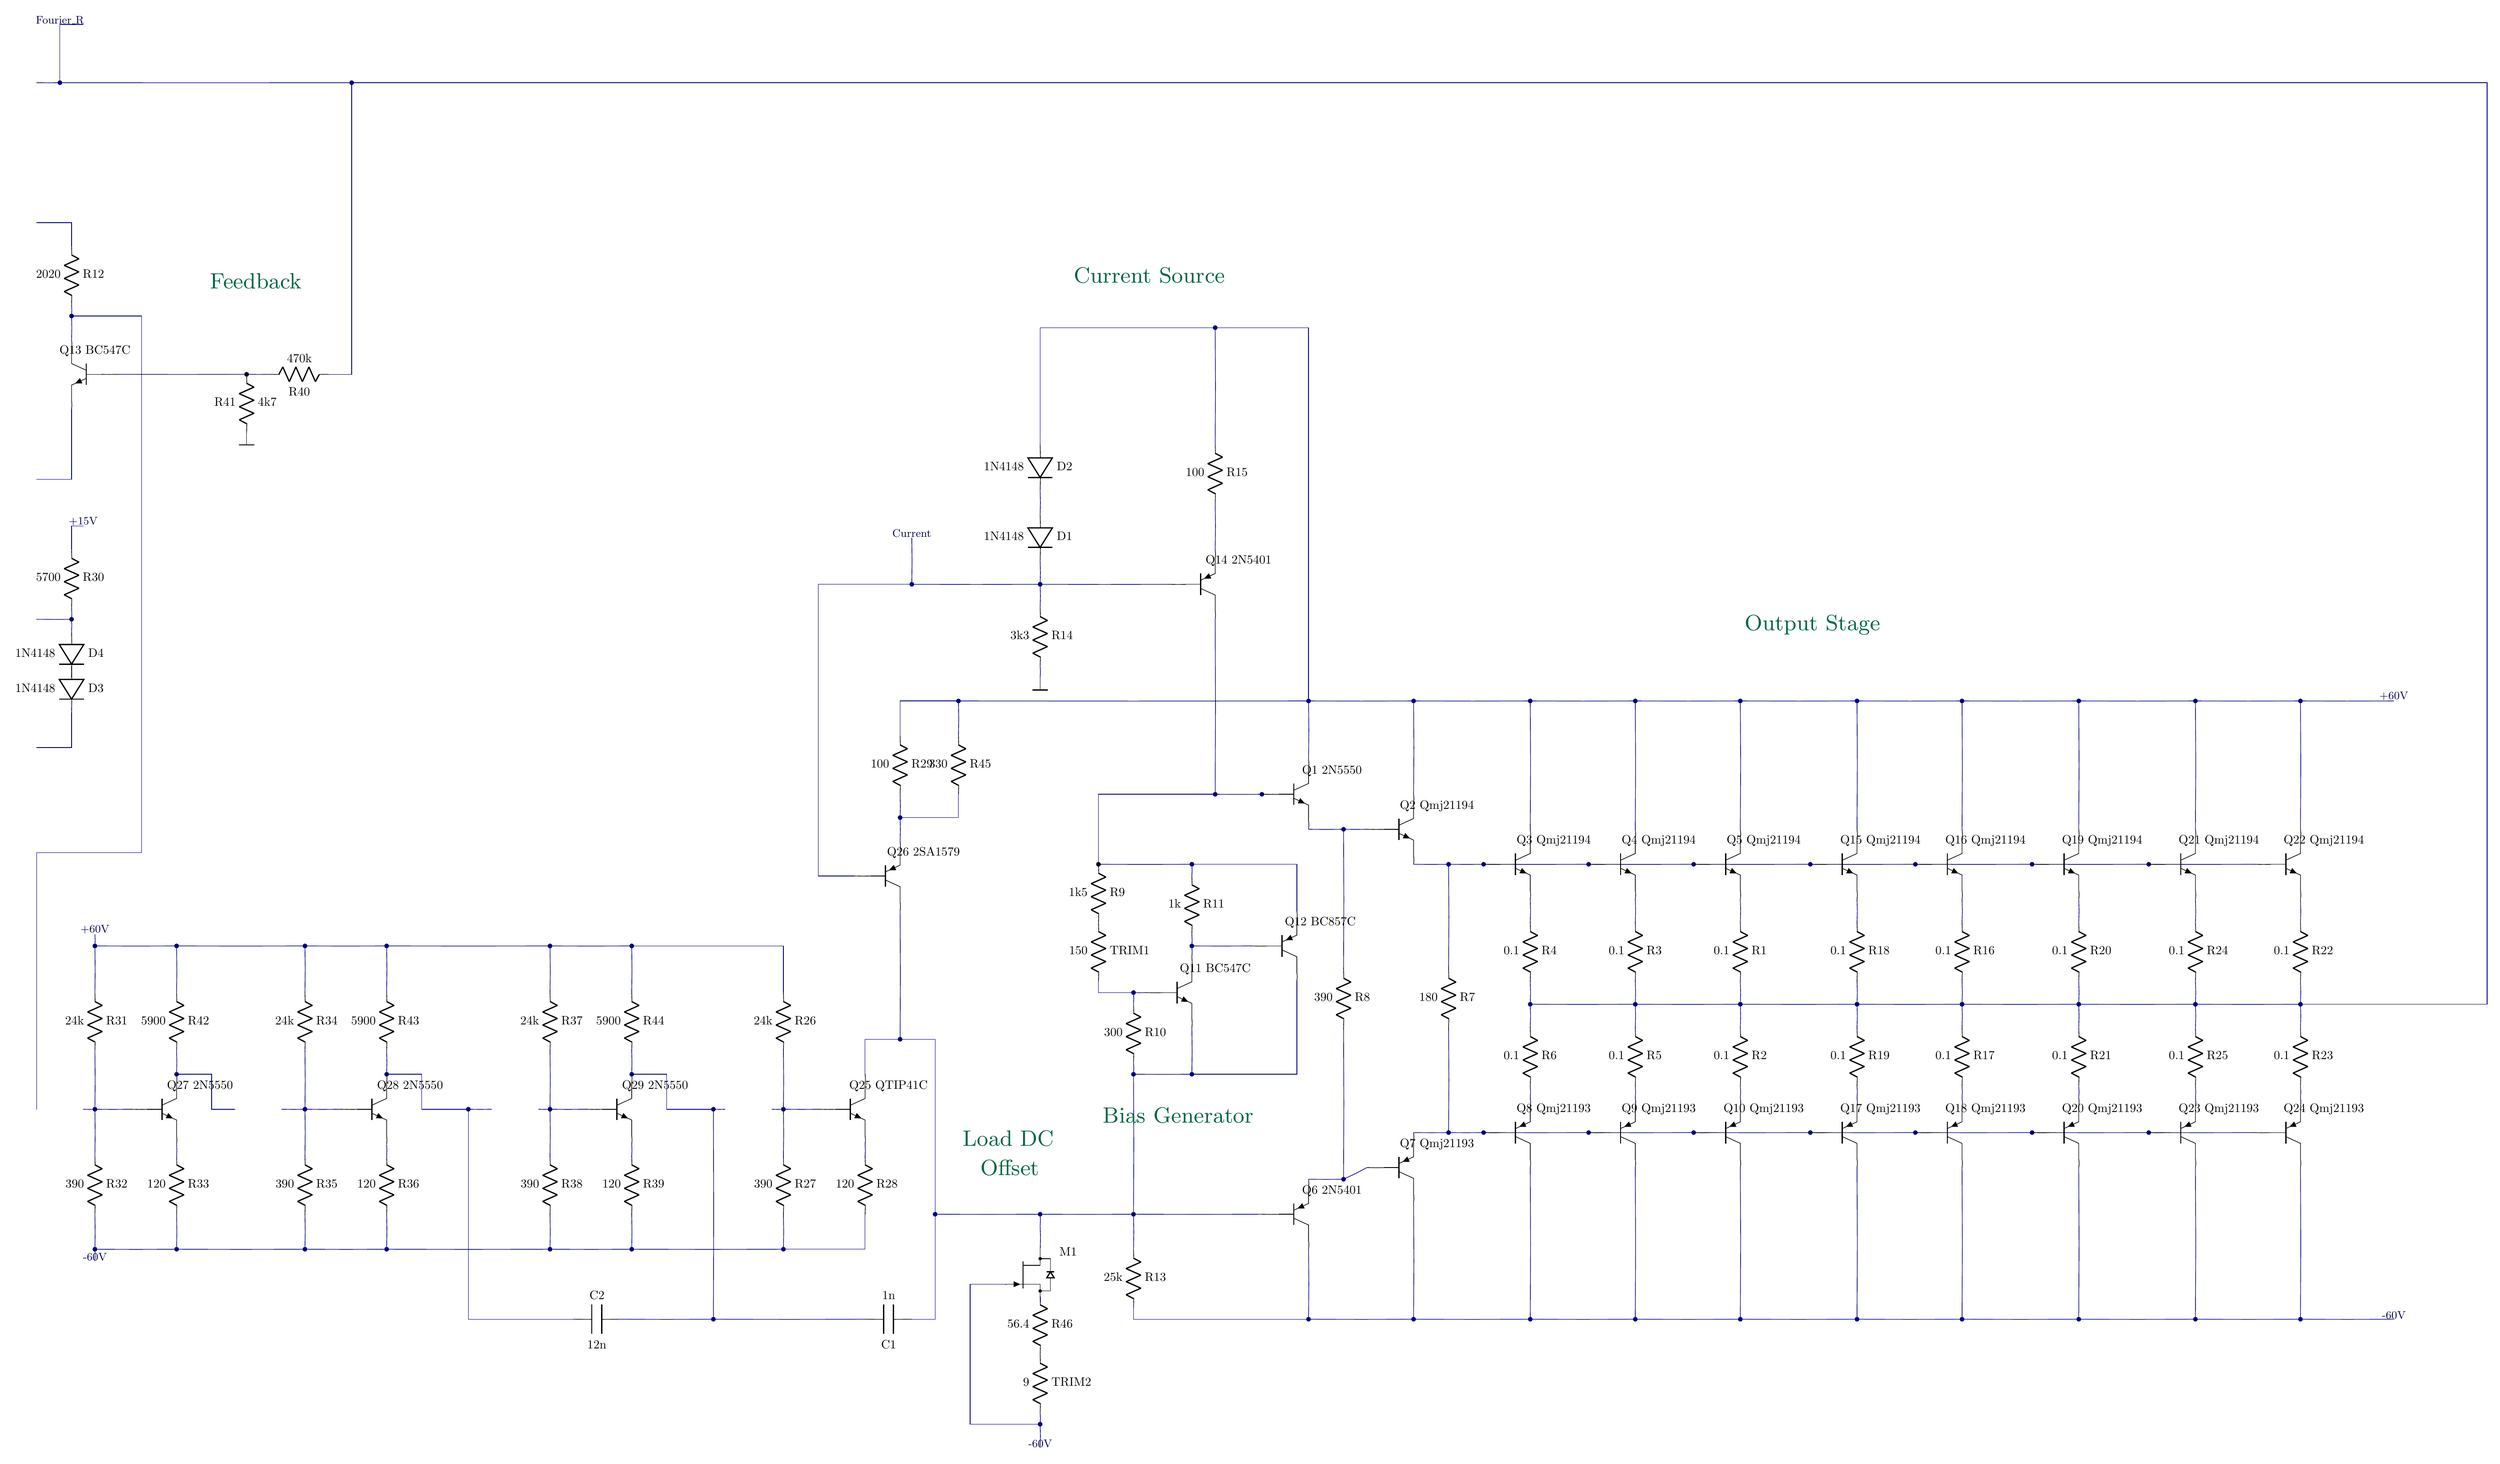
\begin{tikzpicture}[circuit ee IEC, scale=0.6666666667,line width=.5pt]% default: 0.4
	%\tikzstyle{every node}=[font=\small];%
	%\node [draw] at (0.0,0.0) {\pgfkeysvalueof{/tikz/circuitikz/tripoles/op amp/font}};
\draw [/lt2ti/Net](302.5,-128.0)to[*short,-, color=netcolor] (302.5,-128.0);% wire w3_w4 start
\draw [/lt2ti/Net](301.5,-130.5)to[*short,-*, color=netcolor] (301.5,-130.5);% wire w3_w4 end
\draw [/lt2ti/Net](302.5,-128.0) --  (301.5,-128.0) -- (301.5,-130.5); % wire w3_w4 polyline 
\draw [/lt2ti/Net](301.5,-130.5)to[*short,*-, color=netcolor] (300.5,-130.5);% wire w5
\draw [/lt2ti/Net](314.0,-130.5)to[*short,*-*, color=netcolor] (301.5,-130.5);% wire w6
\draw [/lt2ti/Net](314.0,-130.5)to[*short,*-, color=netcolor] (314.0,-130.5);% wire w17_w18 start
\draw [/lt2ti/Net](313.0,-143.0)to[*short,-, color=netcolor] (313.0,-143.0);% wire w17_w18 end
\draw [/lt2ti/Net](314.0,-130.5) --  (314.0,-143.0) -- (313.0,-143.0); % wire w17_w18 polyline 
\draw [/lt2ti/Net](302.0,-137.5)to[*short,-, color=netcolor] (302.0,-137.5);% wire w8_w9 start
\draw [/lt2ti/Net](300.5,-136.5)to[*short,-, color=netcolor] (300.5,-136.5);% wire w8_w9 end
\draw [/lt2ti/Net](302.0,-137.5) --  (302.0,-136.5) -- (300.5,-136.5); % wire w8_w9 polyline 
\draw [/lt2ti/Net](302.0,-140.5)to[*short,*-, color=netcolor] (302.0,-140.0);% wire w10
\draw [/lt2ti/Net](351.0,-141.0)to[*short,*-, color=netcolor] (351.0,-141.0);% wire w12_w19 start
\draw [/lt2ti/Net](343.5,-146.0)to[*short,-, color=netcolor] (343.5,-146.0);% wire w12_w19 end
\draw [/lt2ti/Net](351.0,-141.0) --  (343.5,-141.0) -- (343.5,-146.0); % wire w12_w19 polyline 
\draw [/lt2ti/Net](302.0,-141.5)to[*short,-*, color=netcolor] (302.0,-140.5);% wire w14
\draw [/lt2ti/Net](309.5,-143.0)to[*short,*-, color=netcolor] (304.0,-143.0);% wire w15
\draw [/lt2ti/Net](310.5,-143.0)to[*short,-*, color=netcolor] (309.5,-143.0);% wire w16
\draw [/lt2ti/Net](351.0,-146.0)to[*short,-*, color=netcolor] (351.0,-141.0);% wire w20
\draw [/lt2ti/Net](302.0,-144.5)to[*short,-, color=netcolor] (302.0,-144.5);% wire w21_w22 start
\draw [/lt2ti/Net](300.5,-147.5)to[*short,-, color=netcolor] (300.5,-147.5);% wire w21_w22 end
\draw [/lt2ti/Net](302.0,-144.5) --  (302.0,-147.5) -- (300.5,-147.5); % wire w21_w22 polyline 
\draw [/lt2ti/Net](343.5,-149.0)to[*short,-, color=netcolor] (343.5,-148.0);% wire w23
\draw [/lt2ti/Net](302.5,-149.5)to[*short,-, color=netcolor] (302.5,-149.5);% wire w24_w25 start
\draw [/lt2ti/Net](302.0,-150.5)to[*short,-, color=netcolor] (302.0,-150.5);% wire w24_w25 end
\draw [/lt2ti/Net](302.5,-149.5) --  (302.0,-149.5) -- (302.0,-150.5); % wire w24_w25 polyline 
\draw [/lt2ti/Net](351.0,-150.5)to[*short,-, color=netcolor] (351.0,-148.5);% wire w26
\draw [/lt2ti/Net](338.0,-152.0)to[*short,*-, color=netcolor] (338.0,-150.0);% wire w27
\draw [/lt2ti/Net](343.5,-152.0)to[*short,*-, color=netcolor] (343.5,-151.0);% wire w29
\draw [/lt2ti/Net](343.5,-152.0)to[*short,*-*, color=netcolor] (338.0,-152.0);% wire w30
\draw [/lt2ti/Net](349.0,-152.0)to[*short,-*, color=netcolor] (343.5,-152.0);% wire w31
\draw [/lt2ti/Net](343.5,-153.0)to[*short,-*, color=netcolor] (343.5,-152.0);% wire w32
\draw [/lt2ti/Net](302.0,-153.5)to[*short,*-, color=netcolor] (302.0,-153.0);% wire w33
\draw [/lt2ti/Net](302.0,-153.5)to[*short,*-, color=netcolor] (300.5,-153.5);% wire w34
\draw [/lt2ti/Net](302.0,-154.0)to[*short,-*, color=netcolor] (302.0,-153.5);% wire w35
\draw [/lt2ti/Net](302.0,-156.0)to[*short,-, color=netcolor] (302.0,-155.5);% wire w36
\draw [/lt2ti/Net](343.5,-156.0)to[*short,-, color=netcolor] (343.5,-155.5);% wire w37
\draw [/lt2ti/Net](340.0,-157.0)to[*short,*-, color=netcolor] (340.0,-157.0);% wire w38_w51 start
\draw [/lt2ti/Net](337.5,-158.5)to[*short,-, color=netcolor] (337.5,-158.5);% wire w38_w51 end
\draw [/lt2ti/Net](340.0,-157.0) --  (337.5,-157.0) -- (337.5,-158.5); % wire w38_w51 polyline 
\draw [/lt2ti/Net](355.0,-157.0)to[*short,*-*, color=netcolor] (340.0,-157.0);% wire w40
\draw [/lt2ti/Net](355.0,-157.0)to[*short,*-, color=netcolor] (355.0,-157.0);% wire w13_w39 start
\draw [/lt2ti/Net](351.0,-141.0)to[*short,-*, color=netcolor] (351.0,-141.0);% wire w13_w39 end
\draw [/lt2ti/Net](355.0,-157.0) --  (355.0,-141.0) -- (351.0,-141.0); % wire w13_w39 polyline 
\draw [/lt2ti/Net](359.5,-157.0)to[*short,*-*, color=netcolor] (355.0,-157.0);% wire w41
\draw [/lt2ti/Net](364.5,-157.0)to[*short,*-*, color=netcolor] (359.5,-157.0);% wire w42
\draw [/lt2ti/Net](369.0,-157.0)to[*short,*-*, color=netcolor] (364.5,-157.0);% wire w43
\draw [/lt2ti/Net](373.5,-157.0)to[*short,*-*, color=netcolor] (369.0,-157.0);% wire w44
\draw [/lt2ti/Net](378.5,-157.0)to[*short,*-*, color=netcolor] (373.5,-157.0);% wire w45
\draw [/lt2ti/Net](383.0,-157.0)to[*short,*-*, color=netcolor] (378.5,-157.0);% wire w46
\draw [/lt2ti/Net](388.0,-157.0)to[*short,*-*, color=netcolor] (383.0,-157.0);% wire w47
\draw [/lt2ti/Net](393.0,-157.0)to[*short,*-*, color=netcolor] (388.0,-157.0);% wire w48
\draw [/lt2ti/Net](397.5,-157.0)to[*short,*-*, color=netcolor] (393.0,-157.0);% wire w49
\draw [/lt2ti/Net](401.5,-157.0)to[*short,-*, color=netcolor] (397.5,-157.0);% wire w50
\draw [/lt2ti/Net](340.0,-158.5)to[*short,-*, color=netcolor] (340.0,-157.0);% wire w52
\draw [/lt2ti/Net](302.0,-157.5)to[*short,-, color=netcolor] (302.0,-157.5);% wire w53_w54 start
\draw [/lt2ti/Net](300.5,-159.0)to[*short,-, color=netcolor] (300.5,-159.0);% wire w53_w54 end
\draw [/lt2ti/Net](302.0,-157.5) --  (302.0,-159.0) -- (300.5,-159.0); % wire w53_w54 polyline 
\draw [/lt2ti/Net](355.0,-159.5)to[*short,-*, color=netcolor] (355.0,-157.0);% wire w55
\draw [/lt2ti/Net](351.0,-161.0)to[*short,*-, color=netcolor] (351.0,-153.5);% wire w56
\draw [/lt2ti/Net](351.0,-161.0)to[*short,*-, color=netcolor] (351.0,-161.0);% wire w57_w77 start
\draw [/lt2ti/Net](346.0,-164.0)to[*short,-*, color=netcolor] (346.0,-164.0);% wire w57_w77 end
\draw [/lt2ti/Net](351.0,-161.0) --  (346.0,-161.0) -- (346.0,-164.0); % wire w57_w77 polyline 
\draw [/lt2ti/Net](353.0,-161.0)to[*short,*-*, color=netcolor] (351.0,-161.0);% wire w58
\draw [/lt2ti/Net](353.5,-161.0)to[*short,-*, color=netcolor] (353.0,-161.0);% wire w59
\draw [/lt2ti/Net](359.5,-161.0)to[*short,-*, color=netcolor] (359.5,-157.0);% wire w60
\draw [/lt2ti/Net](337.5,-162.0)to[*short,*-, color=netcolor] (337.5,-161.0);% wire w61
\draw [/lt2ti/Net](340.0,-161.0)to[*short,-, color=netcolor] (340.0,-161.0);% wire w62_w63 start
\draw [/lt2ti/Net](337.5,-162.0)to[*short,-*, color=netcolor] (337.5,-162.0);% wire w62_w63 end
\draw [/lt2ti/Net](340.0,-161.0) --  (340.0,-162.0) -- (337.5,-162.0); % wire w62_w63 polyline 
\draw [/lt2ti/Net](356.5,-162.5)to[*short,*-, color=netcolor] (355.0,-162.5);% wire w64
\draw [/lt2ti/Net](357.5,-162.5)to[*short,-*, color=netcolor] (356.5,-162.5);% wire w65
\draw [/lt2ti/Net](364.5,-162.5)to[*short,-*, color=netcolor] (364.5,-157.0);% wire w66
\draw [/lt2ti/Net](369.0,-162.5)to[*short,-*, color=netcolor] (369.0,-157.0);% wire w67
\draw [/lt2ti/Net](373.5,-162.5)to[*short,-*, color=netcolor] (373.5,-157.0);% wire w68
\draw [/lt2ti/Net](378.5,-162.5)to[*short,-*, color=netcolor] (378.5,-157.0);% wire w69
\draw [/lt2ti/Net](383.0,-162.5)to[*short,-*, color=netcolor] (383.0,-157.0);% wire w70
\draw [/lt2ti/Net](388.0,-162.5)to[*short,-*, color=netcolor] (388.0,-157.0);% wire w71
\draw [/lt2ti/Net](393.0,-162.5)to[*short,-*, color=netcolor] (393.0,-157.0);% wire w72
\draw [/lt2ti/Net](397.5,-162.5)to[*short,-*, color=netcolor] (397.5,-157.0);% wire w73
\draw [/lt2ti/Net](337.5,-163.0)to[*short,-*, color=netcolor] (337.5,-162.0);% wire w74
\draw [/lt2ti/Net](350.0,-164.0)to[*short,*-*, color=netcolor] (346.0,-164.0);% wire w78
\draw [/lt2ti/Net](361.0,-164.0)to[*short,*-, color=netcolor] (359.5,-164.0);% wire w80
\draw [/lt2ti/Net](362.5,-164.0)to[*short,*-*, color=netcolor] (361.0,-164.0);% wire w81
\draw [/lt2ti/Net](367.0,-164.0)to[*short,*-*, color=netcolor] (362.5,-164.0);% wire w82
\draw [/lt2ti/Net](371.5,-164.0)to[*short,*-*, color=netcolor] (367.0,-164.0);% wire w83
\draw [/lt2ti/Net](376.5,-164.0)to[*short,*-*, color=netcolor] (371.5,-164.0);% wire w84
\draw [/lt2ti/Net](381.0,-164.0)to[*short,*-*, color=netcolor] (376.5,-164.0);% wire w85
\draw [/lt2ti/Net](386.0,-164.0)to[*short,*-*, color=netcolor] (381.0,-164.0);% wire w86
\draw [/lt2ti/Net](391.0,-164.0)to[*short,*-*, color=netcolor] (386.0,-164.0);% wire w87
\draw [/lt2ti/Net](395.5,-164.0)to[*short,-*, color=netcolor] (391.0,-164.0);% wire w88
\draw [/lt2ti/Net](335.5,-164.5)to[*short,-, color=netcolor] (335.5,-164.5);% wire w90_w28_w89 start
\draw [/lt2ti/Net](338.0,-152.0)to[*short,-*, color=netcolor] (338.0,-152.0);% wire w90_w28_w89 end
\draw [/lt2ti/Net](335.5,-164.5) --  (334.0,-164.5) --  (334.0,-152.0) -- (338.0,-152.0); % wire w90_w28_w89 polyline 
\draw [/lt2ti/Net](350.0,-164.5)to[*short,-*, color=netcolor] (350.0,-164.0);% wire w91
\draw [/lt2ti/Net](354.5,-166.0)to[*short,-, color=netcolor] (354.5,-166.0);% wire w79_w92 start
\draw [/lt2ti/Net](350.0,-164.0)to[*short,-*, color=netcolor] (350.0,-164.0);% wire w79_w92 end
\draw [/lt2ti/Net](354.5,-166.0) --  (354.5,-164.0) -- (350.0,-164.0); % wire w79_w92 polyline 
\draw [/lt2ti/Net](364.5,-166.5)to[*short,-, color=netcolor] (364.5,-165.5);% wire w93
\draw [/lt2ti/Net](369.0,-166.5)to[*short,-, color=netcolor] (369.0,-165.5);% wire w94
\draw [/lt2ti/Net](373.5,-166.5)to[*short,-, color=netcolor] (373.5,-165.5);% wire w95
\draw [/lt2ti/Net](378.5,-166.5)to[*short,-, color=netcolor] (378.5,-165.5);% wire w96
\draw [/lt2ti/Net](383.0,-166.5)to[*short,-, color=netcolor] (383.0,-165.5);% wire w97
\draw [/lt2ti/Net](388.0,-166.5)to[*short,-, color=netcolor] (388.0,-165.5);% wire w98
\draw [/lt2ti/Net](393.0,-166.5)to[*short,-, color=netcolor] (393.0,-165.5);% wire w99
\draw [/lt2ti/Net](397.5,-166.5)to[*short,-, color=netcolor] (397.5,-165.5);% wire w100
\draw [/lt2ti/Net](303.0,-167.5)to[*short,*-, color=netcolor] (303.0,-167.0);% wire w101
\draw [/lt2ti/Net](306.5,-167.5)to[*short,*-*, color=netcolor] (303.0,-167.5);% wire w102
\draw [/lt2ti/Net](312.0,-167.5)to[*short,*-*, color=netcolor] (306.5,-167.5);% wire w103
\draw [/lt2ti/Net](315.5,-167.5)to[*short,*-*, color=netcolor] (312.0,-167.5);% wire w104
\draw [/lt2ti/Net](322.5,-167.5)to[*short,*-*, color=netcolor] (315.5,-167.5);% wire w105
\draw [/lt2ti/Net](326.0,-167.5)to[*short,*-*, color=netcolor] (322.5,-167.5);% wire w106
\draw [/lt2ti/Net](350.0,-167.5)to[*short,*-, color=netcolor] (350.0,-167.0);% wire w108
\draw [/lt2ti/Net](352.5,-167.5)to[*short,-*, color=netcolor] (350.0,-167.5);% wire w109
\draw [/lt2ti/Net](350.0,-168.0)to[*short,-*, color=netcolor] (350.0,-167.5);% wire w110
\draw [/lt2ti/Net](356.5,-168.5)to[*short,-*, color=netcolor] (356.5,-162.5);% wire w111
\draw [/lt2ti/Net](361.0,-168.5)to[*short,-*, color=netcolor] (361.0,-164.0);% wire w112
\draw [/lt2ti/Net](303.0,-169.5)to[*short,-*, color=netcolor] (303.0,-167.5);% wire w113
\draw [/lt2ti/Net](306.5,-169.5)to[*short,-*, color=netcolor] (306.5,-167.5);% wire w114
\draw [/lt2ti/Net](312.0,-169.5)to[*short,-*, color=netcolor] (312.0,-167.5);% wire w115
\draw [/lt2ti/Net](315.5,-169.5)to[*short,-*, color=netcolor] (315.5,-167.5);% wire w116
\draw [/lt2ti/Net](322.5,-169.5)to[*short,-*, color=netcolor] (322.5,-167.5);% wire w117
\draw [/lt2ti/Net](326.0,-169.5)to[*short,-*, color=netcolor] (326.0,-167.5);% wire w118
\draw [/lt2ti/Net](332.5,-169.5)to[*short,-, color=netcolor] (332.5,-169.5);% wire w107_w119 start
\draw [/lt2ti/Net](326.0,-167.5)to[*short,-*, color=netcolor] (326.0,-167.5);% wire w107_w119 end
\draw [/lt2ti/Net](332.5,-169.5) --  (332.5,-167.5) -- (326.0,-167.5); % wire w107_w119 polyline 
\draw [/lt2ti/Net](347.5,-169.5)to[*short,*-, color=netcolor] (347.5,-169.5);% wire w120_w121 start
\draw [/lt2ti/Net](346.0,-169.0)to[*short,-, color=netcolor] (346.0,-169.0);% wire w120_w121 end
\draw [/lt2ti/Net](347.5,-169.5) --  (346.0,-169.5) -- (346.0,-169.0); % wire w120_w121 polyline 
\draw [/lt2ti/Net](348.0,-169.5)to[*short,-*, color=netcolor] (347.5,-169.5);% wire w122
\draw [/lt2ti/Net](347.5,-170.0)to[*short,-*, color=netcolor] (347.5,-169.5);% wire w123
\draw [/lt2ti/Net](364.5,-170.0)to[*short,*-, color=netcolor] (364.5,-169.0);% wire w124
\draw [/lt2ti/Net](369.0,-170.0)to[*short,*-, color=netcolor] (369.0,-169.0);% wire w125
\draw [/lt2ti/Net](369.0,-170.0)to[*short,*-*, color=netcolor] (364.5,-170.0);% wire w126
\draw [/lt2ti/Net](373.5,-170.0)to[*short,*-, color=netcolor] (373.5,-169.0);% wire w127
\draw [/lt2ti/Net](373.5,-170.0)to[*short,*-*, color=netcolor] (369.0,-170.0);% wire w128
\draw [/lt2ti/Net](378.5,-170.0)to[*short,*-, color=netcolor] (378.5,-169.0);% wire w129
\draw [/lt2ti/Net](378.5,-170.0)to[*short,*-*, color=netcolor] (373.5,-170.0);% wire w130
\draw [/lt2ti/Net](383.0,-170.0)to[*short,*-, color=netcolor] (383.0,-169.0);% wire w131
\draw [/lt2ti/Net](383.0,-170.0)to[*short,*-*, color=netcolor] (378.5,-170.0);% wire w132
\draw [/lt2ti/Net](388.0,-170.0)to[*short,*-, color=netcolor] (388.0,-169.0);% wire w133
\draw [/lt2ti/Net](388.0,-170.0)to[*short,*-*, color=netcolor] (383.0,-170.0);% wire w134
\draw [/lt2ti/Net](393.0,-170.0)to[*short,*-, color=netcolor] (393.0,-169.0);% wire w135
\draw [/lt2ti/Net](393.0,-170.0)to[*short,*-*, color=netcolor] (388.0,-170.0);% wire w136
\draw [/lt2ti/Net](397.5,-170.0)to[*short,*-, color=netcolor] (397.5,-169.0);% wire w137
\draw [/lt2ti/Net](397.5,-170.0)to[*short,*-*, color=netcolor] (393.0,-170.0);% wire w138
\draw [/lt2ti/Net](397.5,-170.0)to[*short,*-, color=netcolor] (397.5,-170.0);% wire w140_w7_w139 start
\draw [/lt2ti/Net](314.0,-130.5)to[*short,-*, color=netcolor] (314.0,-130.5);% wire w140_w7_w139 end
\draw [/lt2ti/Net](397.5,-170.0) --  (405.5,-170.0) --  (405.5,-130.5) -- (314.0,-130.5); % wire w140_w7_w139 polyline 
\draw [/lt2ti/Net](364.5,-171.0)to[*short,-*, color=netcolor] (364.5,-170.0);% wire w141
\draw [/lt2ti/Net](369.0,-171.0)to[*short,-*, color=netcolor] (369.0,-170.0);% wire w142
\draw [/lt2ti/Net](373.5,-171.0)to[*short,-*, color=netcolor] (373.5,-170.0);% wire w143
\draw [/lt2ti/Net](378.5,-171.0)to[*short,-*, color=netcolor] (378.5,-170.0);% wire w144
\draw [/lt2ti/Net](383.0,-171.0)to[*short,-*, color=netcolor] (383.0,-170.0);% wire w145
\draw [/lt2ti/Net](388.0,-171.0)to[*short,-*, color=netcolor] (388.0,-170.0);% wire w146
\draw [/lt2ti/Net](393.0,-171.0)to[*short,-*, color=netcolor] (393.0,-170.0);% wire w147
\draw [/lt2ti/Net](397.5,-171.0)to[*short,-*, color=netcolor] (397.5,-170.0);% wire w148
\draw [/lt2ti/Net](337.5,-171.5)to[*short,*-, color=netcolor] (337.5,-166.0);% wire w149
\draw [/lt2ti/Net](337.5,-171.5)to[*short,*-, color=netcolor] (337.5,-171.5);% wire w150_w158 start
\draw [/lt2ti/Net](336.0,-173.0)to[*short,-, color=netcolor] (336.0,-173.0);% wire w150_w158 end
\draw [/lt2ti/Net](337.5,-171.5) --  (336.0,-171.5) -- (336.0,-173.0); % wire w150_w158 polyline 
\draw [/lt2ti/Net](306.5,-173.0)to[*short,*-, color=netcolor] (306.5,-172.0);% wire w152
\draw [/lt2ti/Net](315.5,-173.0)to[*short,*-, color=netcolor] (315.5,-172.0);% wire w154
\draw [/lt2ti/Net](326.0,-173.0)to[*short,*-, color=netcolor] (326.0,-172.0);% wire w156
\draw [/lt2ti/Net](347.5,-173.0)to[*short,*-, color=netcolor] (347.5,-172.5);% wire w159
\draw [/lt2ti/Net](350.0,-173.0)to[*short,*-, color=netcolor] (350.0,-171.0);% wire w160
\draw [/lt2ti/Net](350.0,-173.0)to[*short,*-*, color=netcolor] (347.5,-173.0);% wire w161
\draw [/lt2ti/Net](354.5,-169.0)to[*short,-, color=netcolor] (354.5,-169.0);% wire w162_w163 start
\draw [/lt2ti/Net](350.0,-173.0)to[*short,-*, color=netcolor] (350.0,-173.0);% wire w162_w163 end
\draw [/lt2ti/Net](354.5,-169.0) --  (354.5,-173.0) -- (350.0,-173.0); % wire w162_w163 polyline 
\draw [/lt2ti/Net](364.5,-174.0)to[*short,-, color=netcolor] (364.5,-173.5);% wire w164
\draw [/lt2ti/Net](369.0,-174.0)to[*short,-, color=netcolor] (369.0,-173.5);% wire w165
\draw [/lt2ti/Net](373.5,-174.0)to[*short,-, color=netcolor] (373.5,-173.5);% wire w166
\draw [/lt2ti/Net](378.5,-174.0)to[*short,-, color=netcolor] (378.5,-173.5);% wire w167
\draw [/lt2ti/Net](383.0,-174.0)to[*short,-, color=netcolor] (383.0,-173.5);% wire w168
\draw [/lt2ti/Net](388.0,-174.0)to[*short,-, color=netcolor] (388.0,-173.5);% wire w169
\draw [/lt2ti/Net](393.0,-174.0)to[*short,-, color=netcolor] (393.0,-173.5);% wire w170
\draw [/lt2ti/Net](397.5,-174.0)to[*short,-, color=netcolor] (397.5,-173.5);% wire w171
\draw [/lt2ti/Net](300.5,-174.5)to[*short,-, color=netcolor] (300.5,-174.5);% wire w172_w76_w11_w75 start
\draw [/lt2ti/Net](302.0,-140.5)to[*short,-*, color=netcolor] (302.0,-140.5);% wire w172_w76_w11_w75 end
\draw [/lt2ti/Net](300.5,-174.5) --  (300.5,-163.5) --  (305.0,-163.5) --  (305.0,-140.5) -- (302.0,-140.5); % wire w172_w76_w11_w75 polyline 
\draw [/lt2ti/Net](303.0,-174.5)to[*short,*-, color=netcolor] (303.0,-172.0);% wire w173
\draw [/lt2ti/Net](303.0,-174.5)to[*short,*-, color=netcolor] (302.5,-174.5);% wire w174
\draw [/lt2ti/Net](304.5,-174.5)to[*short,-*, color=netcolor] (303.0,-174.5);% wire w175
\draw [/lt2ti/Net](309.0,-174.5)to[*short,-, color=netcolor] (309.0,-174.5);% wire w177_w153_w176 start
\draw [/lt2ti/Net](306.5,-173.0)to[*short,-*, color=netcolor] (306.5,-173.0);% wire w177_w153_w176 end
\draw [/lt2ti/Net](309.0,-174.5) --  (308.0,-174.5) --  (308.0,-173.0) -- (306.5,-173.0); % wire w177_w153_w176 polyline 
\draw [/lt2ti/Net](312.0,-174.5)to[*short,*-, color=netcolor] (312.0,-172.0);% wire w178
\draw [/lt2ti/Net](312.0,-174.5)to[*short,*-, color=netcolor] (311.0,-174.5);% wire w179
\draw [/lt2ti/Net](313.5,-174.5)to[*short,-*, color=netcolor] (312.0,-174.5);% wire w180
\draw [/lt2ti/Net](319.0,-174.5)to[*short,*-, color=netcolor] (319.0,-174.5);% wire w182_w155_w181 start
\draw [/lt2ti/Net](315.5,-173.0)to[*short,-*, color=netcolor] (315.5,-173.0);% wire w182_w155_w181 end
\draw [/lt2ti/Net](319.0,-174.5) --  (317.0,-174.5) --  (317.0,-173.0) -- (315.5,-173.0); % wire w182_w155_w181 polyline 
\draw [/lt2ti/Net](320.0,-174.5)to[*short,-*, color=netcolor] (319.0,-174.5);% wire w183
\draw [/lt2ti/Net](322.5,-174.5)to[*short,*-, color=netcolor] (322.5,-172.0);% wire w184
\draw [/lt2ti/Net](322.5,-174.5)to[*short,*-, color=netcolor] (322.0,-174.5);% wire w185
\draw [/lt2ti/Net](324.0,-174.5)to[*short,-*, color=netcolor] (322.5,-174.5);% wire w186
\draw [/lt2ti/Net](329.5,-174.5)to[*short,*-, color=netcolor] (329.5,-174.5);% wire w188_w157_w187 start
\draw [/lt2ti/Net](326.0,-173.0)to[*short,-*, color=netcolor] (326.0,-173.0);% wire w188_w157_w187 end
\draw [/lt2ti/Net](329.5,-174.5) --  (327.5,-174.5) --  (327.5,-173.0) -- (326.0,-173.0); % wire w188_w157_w187 polyline 
\draw [/lt2ti/Net](330.0,-174.5)to[*short,-*, color=netcolor] (329.5,-174.5);% wire w189
\draw [/lt2ti/Net](332.5,-174.5)to[*short,*-, color=netcolor] (332.5,-172.0);% wire w190
\draw [/lt2ti/Net](332.5,-174.5)to[*short,*-, color=netcolor] (332.0,-174.5);% wire w191
\draw [/lt2ti/Net](334.0,-174.5)to[*short,-*, color=netcolor] (332.5,-174.5);% wire w192
\draw [/lt2ti/Net](361.0,-175.5)to[*short,*-, color=netcolor] (361.0,-171.0);% wire w193
\draw [/lt2ti/Net](361.0,-175.5)to[*short,*-, color=netcolor] (359.5,-175.5);% wire w194
\draw [/lt2ti/Net](362.5,-175.5)to[*short,*-*, color=netcolor] (361.0,-175.5);% wire w195
\draw [/lt2ti/Net](367.0,-175.5)to[*short,*-*, color=netcolor] (362.5,-175.5);% wire w196
\draw [/lt2ti/Net](371.5,-175.5)to[*short,*-*, color=netcolor] (367.0,-175.5);% wire w197
\draw [/lt2ti/Net](376.5,-175.5)to[*short,*-*, color=netcolor] (371.5,-175.5);% wire w198
\draw [/lt2ti/Net](381.0,-175.5)to[*short,*-*, color=netcolor] (376.5,-175.5);% wire w199
\draw [/lt2ti/Net](386.0,-175.5)to[*short,*-*, color=netcolor] (381.0,-175.5);% wire w200
\draw [/lt2ti/Net](391.0,-175.5)to[*short,*-*, color=netcolor] (386.0,-175.5);% wire w201
\draw [/lt2ti/Net](395.5,-175.5)to[*short,-*, color=netcolor] (391.0,-175.5);% wire w202
\draw [/lt2ti/Net](303.0,-176.5)to[*short,-*, color=netcolor] (303.0,-174.5);% wire w203
\draw [/lt2ti/Net](306.5,-176.5)to[*short,-, color=netcolor] (306.5,-176.0);% wire w204
\draw [/lt2ti/Net](312.0,-176.5)to[*short,-*, color=netcolor] (312.0,-174.5);% wire w205
\draw [/lt2ti/Net](315.5,-176.5)to[*short,-, color=netcolor] (315.5,-176.0);% wire w206
\draw [/lt2ti/Net](322.5,-176.5)to[*short,-*, color=netcolor] (322.5,-174.5);% wire w207
\draw [/lt2ti/Net](326.0,-176.5)to[*short,-, color=netcolor] (326.0,-176.0);% wire w208
\draw [/lt2ti/Net](332.5,-176.5)to[*short,-*, color=netcolor] (332.5,-174.5);% wire w209
\draw [/lt2ti/Net](336.0,-176.5)to[*short,-, color=netcolor] (336.0,-176.0);% wire w210
\draw [/lt2ti/Net](356.5,-177.5)to[*short,*-, color=netcolor] (356.5,-171.0);% wire w211
\draw [/lt2ti/Net](356.5,-177.5)to[*short,*-, color=netcolor] (357.5,-177.0);% wire w212
\draw [/lt2ti/Net](356.5,-177.5)to[*short,*-, color=netcolor] (355.0,-177.5);% wire w213
\draw [/lt2ti/Net](339.0,-179.0)to[*short,*-, color=netcolor] (339.0,-179.0);% wire w151_w214 start
\draw [/lt2ti/Net](337.5,-171.5)to[*short,-*, color=netcolor] (337.5,-171.5);% wire w151_w214 end
\draw [/lt2ti/Net](339.0,-179.0) --  (339.0,-171.5) -- (337.5,-171.5); % wire w151_w214 polyline 
\draw [/lt2ti/Net](339.0,-179.0)to[*short,*-, color=netcolor] (339.0,-179.0);% wire w243_w244 start
\draw [/lt2ti/Net](338.0,-183.5)to[*short,-, color=netcolor] (338.0,-183.5);% wire w243_w244 end
\draw [/lt2ti/Net](339.0,-179.0) --  (339.0,-183.5) -- (338.0,-183.5); % wire w243_w244 polyline 
\draw [/lt2ti/Net](343.5,-179.0)to[*short,*-*, color=netcolor] (339.0,-179.0);% wire w215
\draw [/lt2ti/Net](347.5,-179.0)to[*short,*-*, color=netcolor] (347.5,-173.0);% wire w216
\draw [/lt2ti/Net](347.5,-179.0)to[*short,*-*, color=netcolor] (343.5,-179.0);% wire w217
\draw [/lt2ti/Net](353.0,-179.0)to[*short,-*, color=netcolor] (347.5,-179.0);% wire w218
\draw [/lt2ti/Net](343.5,-179.5)to[*short,-*, color=netcolor] (343.5,-179.0);% wire w219
\draw [/lt2ti/Net](303.0,-180.5)to[*short,*-, color=netcolor] (303.0,-179.0);% wire w220
\draw [/lt2ti/Net](306.5,-180.5)to[*short,*-, color=netcolor] (306.5,-179.0);% wire w221
\draw [/lt2ti/Net](306.5,-180.5)to[*short,*-*, color=netcolor] (303.0,-180.5);% wire w222
\draw [/lt2ti/Net](312.0,-180.5)to[*short,*-, color=netcolor] (312.0,-179.0);% wire w223
\draw [/lt2ti/Net](312.0,-180.5)to[*short,*-*, color=netcolor] (306.5,-180.5);% wire w224
\draw [/lt2ti/Net](315.5,-180.5)to[*short,*-, color=netcolor] (315.5,-179.0);% wire w225
\draw [/lt2ti/Net](315.5,-180.5)to[*short,*-*, color=netcolor] (312.0,-180.5);% wire w226
\draw [/lt2ti/Net](322.5,-180.5)to[*short,*-, color=netcolor] (322.5,-179.0);% wire w227
\draw [/lt2ti/Net](322.5,-180.5)to[*short,*-*, color=netcolor] (315.5,-180.5);% wire w228
\draw [/lt2ti/Net](326.0,-180.5)to[*short,*-, color=netcolor] (326.0,-179.0);% wire w229
\draw [/lt2ti/Net](326.0,-180.5)to[*short,*-*, color=netcolor] (322.5,-180.5);% wire w230
\draw [/lt2ti/Net](332.5,-180.5)to[*short,*-, color=netcolor] (332.5,-179.0);% wire w231
\draw [/lt2ti/Net](332.5,-180.5)to[*short,*-*, color=netcolor] (326.0,-180.5);% wire w232
\draw [/lt2ti/Net](336.0,-179.0)to[*short,-, color=netcolor] (336.0,-179.0);% wire w233_w234 start
\draw [/lt2ti/Net](332.5,-180.5)to[*short,-*, color=netcolor] (332.5,-180.5);% wire w233_w234 end
\draw [/lt2ti/Net](336.0,-179.0) --  (336.0,-180.5) -- (332.5,-180.5); % wire w233_w234 polyline 
\draw [/lt2ti/Net](347.5,-180.5)to[*short,-*, color=netcolor] (347.5,-179.0);% wire w235
\draw [/lt2ti/Net](303.0,-181.0)to[*short,-*, color=netcolor] (303.0,-180.5);% wire w236
\draw [/lt2ti/Net](323.5,-183.5)to[*short,-, color=netcolor] (323.5,-183.5);% wire w238_w239 start
\draw [/lt2ti/Net](319.0,-174.5)to[*short,-*, color=netcolor] (319.0,-174.5);% wire w238_w239 end
\draw [/lt2ti/Net](323.5,-183.5) --  (319.0,-183.5) -- (319.0,-174.5); % wire w238_w239 polyline 
\draw [/lt2ti/Net](329.5,-183.5)to[*short,*-*, color=netcolor] (329.5,-174.5);% wire w240
\draw [/lt2ti/Net](329.5,-183.5)to[*short,*-, color=netcolor] (325.5,-183.5);% wire w241
\draw [/lt2ti/Net](336.0,-183.5)to[*short,-*, color=netcolor] (329.5,-183.5);% wire w242
\draw [/lt2ti/Net](355.0,-183.5)to[*short,*-, color=netcolor] (355.0,-180.5);% wire w246
\draw [/lt2ti/Net](355.0,-183.5)to[*short,*-, color=netcolor] (355.0,-183.5);% wire w245_w247 start
\draw [/lt2ti/Net](347.5,-183.0)to[*short,-, color=netcolor] (347.5,-183.0);% wire w245_w247 end
\draw [/lt2ti/Net](355.0,-183.5) --  (347.5,-183.5) -- (347.5,-183.0); % wire w245_w247 polyline 
\draw [/lt2ti/Net](359.5,-183.5)to[*short,*-, color=netcolor] (359.5,-178.5);% wire w248
\draw [/lt2ti/Net](359.5,-183.5)to[*short,*-*, color=netcolor] (355.0,-183.5);% wire w249
\draw [/lt2ti/Net](364.5,-183.5)to[*short,*-, color=netcolor] (364.5,-177.0);% wire w250
\draw [/lt2ti/Net](364.5,-183.5)to[*short,*-*, color=netcolor] (359.5,-183.5);% wire w251
\draw [/lt2ti/Net](369.0,-183.5)to[*short,*-, color=netcolor] (369.0,-177.0);% wire w252
\draw [/lt2ti/Net](369.0,-183.5)to[*short,*-*, color=netcolor] (364.5,-183.5);% wire w253
\draw [/lt2ti/Net](373.5,-183.5)to[*short,*-, color=netcolor] (373.5,-177.0);% wire w254
\draw [/lt2ti/Net](373.5,-183.5)to[*short,*-*, color=netcolor] (369.0,-183.5);% wire w255
\draw [/lt2ti/Net](378.5,-183.5)to[*short,*-, color=netcolor] (378.5,-177.0);% wire w256
\draw [/lt2ti/Net](378.5,-183.5)to[*short,*-*, color=netcolor] (373.5,-183.5);% wire w257
\draw [/lt2ti/Net](383.0,-183.5)to[*short,*-, color=netcolor] (383.0,-177.0);% wire w258
\draw [/lt2ti/Net](383.0,-183.5)to[*short,*-*, color=netcolor] (378.5,-183.5);% wire w259
\draw [/lt2ti/Net](388.0,-183.5)to[*short,*-, color=netcolor] (388.0,-177.0);% wire w260
\draw [/lt2ti/Net](388.0,-183.5)to[*short,*-*, color=netcolor] (383.0,-183.5);% wire w261
\draw [/lt2ti/Net](393.0,-183.5)to[*short,*-, color=netcolor] (393.0,-177.0);% wire w262
\draw [/lt2ti/Net](393.0,-183.5)to[*short,*-*, color=netcolor] (388.0,-183.5);% wire w263
\draw [/lt2ti/Net](397.5,-183.5)to[*short,*-, color=netcolor] (397.5,-177.0);% wire w264
\draw [/lt2ti/Net](397.5,-183.5)to[*short,*-*, color=netcolor] (393.0,-183.5);% wire w265
\draw [/lt2ti/Net](401.5,-183.5)to[*short,-*, color=netcolor] (397.5,-183.5);% wire w266
\draw [/lt2ti/Net](343.5,-188.0)to[*short,*-, color=netcolor] (343.5,-187.5);% wire w268
\draw [/lt2ti/Net](343.5,-188.0)to[*short,*-, color=netcolor] (343.5,-188.0);% wire w269_w237_w267 start
\draw [/lt2ti/Net](342.0,-182.0)to[*short,-, color=netcolor] (342.0,-182.0);% wire w269_w237_w267 end
\draw [/lt2ti/Net](343.5,-188.0) --  (340.5,-188.0) --  (340.5,-182.0) -- (342.0,-182.0); % wire w269_w237_w267 polyline 
\draw [/lt2ti/Net](343.5,-189.0)to[*short,-*, color=netcolor] (343.5,-188.0);% wire w270
 \draw (343.5, -156.0) node[rground, xscale=1, yscale=1, rotate=0, ] (undefined) {};%  (undefined)++(0.0,0.0) node {undefined }; % component "circuiTikz\gnd" "undefined" 
 \draw (309.5, -145.5) node[rground, xscale=1, yscale=1, rotate=0, ] (undefined) {};%  (undefined)++(0.0,0.0) node {undefined }; % component "circuiTikz\gnd" "undefined" 
 \draw (355.0, -161.0) node[npn, nobodydiode, , rotate=0, ] (Q1) {}   (Q1)++(1.0,1) node {Q1 2N5550}; % component "npn" "Q1" 
 \draw (353.0, -161.0) to [*short, -] (Q1.B); \draw (355.0, -162.5) to [*short, -] (Q1.E); \draw (355.0, -159.5) to [*short, -] (Q1.C);% extend wires to the connection points   % component "npn" "Q1" 
 \draw (359.5, -162.5) node[npn, nobodydiode, , rotate=0, ] (Q2) {}   (Q2)++(1.0,1) node {Q2 Qmj21194}; % component "npn" "Q2" 
 \draw (357.5, -162.5) to [*short, -] (Q2.B); \draw (359.5, -164.0) to [*short, -] (Q2.E); \draw (359.5, -161.0) to [*short, -] (Q2.C);% extend wires to the connection points   % component "npn" "Q2" 
 \draw (364.5, -164.0) node[npn, nobodydiode, , rotate=0, ] (Q3) {}   (Q3)++(1.0,1) node {Q3 Qmj21194}; % component "npn" "Q3" 
 \draw (362.5, -164.0) to [*short, -] (Q3.B); \draw (364.5, -165.5) to [*short, -] (Q3.E); \draw (364.5, -162.5) to [*short, -] (Q3.C);% extend wires to the connection points   % component "npn" "Q3" 
 \draw (369.0, -164.0) node[npn, nobodydiode, , rotate=0, ] (Q4) {}   (Q4)++(1.0,1) node {Q4 Qmj21194}; % component "npn" "Q4" 
 \draw (367.0, -164.0) to [*short, -] (Q4.B); \draw (369.0, -165.5) to [*short, -] (Q4.E); \draw (369.0, -162.5) to [*short, -] (Q4.C);% extend wires to the connection points   % component "npn" "Q4" 
 \draw (373.5, -164.0) node[npn, nobodydiode, , rotate=0, ] (Q5) {}   (Q5)++(1.0,1) node {Q5 Qmj21194}; % component "npn" "Q5" 
 \draw (371.5, -164.0) to [*short, -] (Q5.B); \draw (373.5, -165.5) to [*short, -] (Q5.E); \draw (373.5, -162.5) to [*short, -] (Q5.C);% extend wires to the connection points   % component "npn" "Q5" 
 \draw (355.0, -179.0) node[pnp, nobodydiode, xscale=1, yscale=1, rotate=0, ] (Q6) {}   (Q6)++(1.0,1) node {Q6 2N5401}; % component "pnp" "Q6" 
 \draw (353.0, -179.0) to [*short, -] (Q6.B); \draw (355.0, -177.5) to [*short, -] (Q6.E); \draw (355.0, -180.5) to [*short, -] (Q6.C);% extend wires to the connection points   % component "pnp" "Q6" 
 \draw (359.5, -177.0) node[pnp, nobodydiode, xscale=1, yscale=1, rotate=0, ] (Q7) {}   (Q7)++(1.0,1) node {Q7 Qmj21193}; % component "pnp" "Q7" 
 \draw (357.5, -177.0) to [*short, -] (Q7.B); \draw (359.5, -175.5) to [*short, -] (Q7.E); \draw (359.5, -178.5) to [*short, -] (Q7.C);% extend wires to the connection points   % component "pnp" "Q7" 
 \draw (364.5, -175.5) node[pnp, nobodydiode, xscale=1, yscale=1, rotate=0, ] (Q8) {}   (Q8)++(1.0,1) node {Q8 Qmj21193}; % component "pnp" "Q8" 
 \draw (362.5, -175.5) to [*short, -] (Q8.B); \draw (364.5, -174.0) to [*short, -] (Q8.E); \draw (364.5, -177.0) to [*short, -] (Q8.C);% extend wires to the connection points   % component "pnp" "Q8" 
 \draw (369.0, -175.5) node[pnp, nobodydiode, xscale=1, yscale=1, rotate=0, ] (Q9) {}   (Q9)++(1.0,1) node {Q9 Qmj21193}; % component "pnp" "Q9" 
 \draw (367.0, -175.5) to [*short, -] (Q9.B); \draw (369.0, -174.0) to [*short, -] (Q9.E); \draw (369.0, -177.0) to [*short, -] (Q9.C);% extend wires to the connection points   % component "pnp" "Q9" 
 \draw (373.5, -175.5) node[pnp, nobodydiode, xscale=1, yscale=1, rotate=0, ] (Q10) {}   (Q10)++(1.0,1) node {Q10 Qmj21193}; % component "pnp" "Q10" 
 \draw (371.5, -175.5) to [*short, -] (Q10.B); \draw (373.5, -174.0) to [*short, -] (Q10.E); \draw (373.5, -177.0) to [*short, -] (Q10.C);% extend wires to the connection points   % component "pnp" "Q10" 
  \draw (373.5, -166.5) to[*resistor, l^=R1, a_=0.1, -, ] (373.5,-169.0){}; %\node [] at (373.0,-166.0) {x}; % component "res" "R1" 
  \draw (373.5, -171.0) to[*resistor, l^=R2, a_=0.1, -, ] (373.5,-173.5){}; %\node [] at (373.0,-170.5) {x}; % component "res" "R2" 
  \draw (369.0, -166.5) to[*resistor, l^=R3, a_=0.1, -, ] (369.0,-169.0){}; %\node [] at (368.5,-166.0) {x}; % component "res" "R3" 
  \draw (364.5, -166.5) to[*resistor, l^=R4, a_=0.1, -, ] (364.5,-169.0){}; %\node [] at (364.0,-166.0) {x}; % component "res" "R4" 
  \draw (369.0, -171.0) to[*resistor, l^=R5, a_=0.1, -, ] (369.0,-173.5){}; %\node [] at (368.5,-170.5) {x}; % component "res" "R5" 
  \draw (364.5, -171.0) to[*resistor, l^=R6, a_=0.1, -, ] (364.5,-173.5){}; %\node [] at (364.0,-170.5) {x}; % component "res" "R6" 
  \draw (361.0, -168.5) to[*resistor, l^=R7, a_=180, -, ] (361.0,-171.0){}; %\node [] at (360.5,-168.0) {x}; % component "res" "R7" 
  \draw (356.5, -168.5) to[*resistor, l^=R8, a_=390, -, ] (356.5,-171.0){}; %\node [] at (356.0,-168.0) {x}; % component "res" "R8" 
 \draw (350.0, -169.5) node[npn, nobodydiode, , rotate=0, ] (Q11) {}   (Q11)++(1.0,1) node {Q11 BC547C}; % component "npn" "Q11" 
 \draw (348.0, -169.5) to [*short, -] (Q11.B); \draw (350.0, -171.0) to [*short, -] (Q11.E); \draw (350.0, -168.0) to [*short, -] (Q11.C);% extend wires to the connection points   % component "npn" "Q11" 
  \draw (346.0, -164.0) to[*resistor, l^=R9, a_=1k5, *-, ] (346.0,-166.5){}; %\node [] at (345.5,-163.5) {x}; % component "res" "R9" 
  \draw (347.5, -170.0) to[*resistor, l^=R10, a_=300, -, ] (347.5,-172.5){}; %\node [] at (347.0,-169.5) {x}; % component "res" "R10" 
  \draw (350.0, -164.5) to[*resistor, l^=R11, a_=1k, -, ] (350.0,-167.0){}; %\node [] at (349.5,-164.0) {x}; % component "res" "R11" 
 \draw (354.5, -167.5) node[pnp, nobodydiode, xscale=1, yscale=1, rotate=0, ] (Q12) {}   (Q12)++(1.0,1) node {Q12 BC857C}; % component "pnp" "Q12" 
 \draw (352.5, -167.5) to [*short, -] (Q12.B); \draw (354.5, -166.0) to [*short, -] (Q12.E); \draw (354.5, -169.0) to [*short, -] (Q12.C);% extend wires to the connection points   % component "pnp" "Q12" 
 \draw (302.0, -143.0) node[npn, nobodydiode, xscale=-1, rotate=0, ] (Q13) {}   (Q13)++(1.0,1) node {Q13 BC547C}; % component "npn" "Q13" 
 \draw (304.0, -143.0) to [*short, -] (Q13.B); \draw (302.0, -144.5) to [*short, -] (Q13.E); \draw (302.0, -141.5) to [*short, -] (Q13.C);% extend wires to the connection points   % component "npn" "Q13" 
  \draw (302.0, -137.5) to[*resistor, l^=R12, a_=2020, -, ] (302.0,-140.0){}; %\node [] at (302.5,-137.0) {x}; % component "res" "R12" 
  \draw (347.5, -180.5) to[*resistor, l^=R13, a_=25k, -, ] (347.5,-183.0){}; %\node [] at (347.0,-180.0) {x}; % component "res" "R13" 
 \draw (351.0, -152.0) node[pnp, nobodydiode, xscale=1, yscale=1, rotate=0, ] (Q14) {}   (Q14)++(1.0,1) node {Q14 2N5401}; % component "pnp" "Q14" 
 \draw (349.0, -152.0) to [*short, -] (Q14.B); \draw (351.0, -150.5) to [*short, -] (Q14.E); \draw (351.0, -153.5) to [*short, -] (Q14.C);% extend wires to the connection points   % component "pnp" "Q14" 
  \draw (343.5, -153.0) to[*resistor, l^=R14, a_=3k3, -, ] (343.5,-155.5){}; %\node [] at (343.0,-152.5) {x}; % component "res" "R14" 
  \draw (343.5, -149.0) to[*diode, l^=D1, a_=1N4148, ] (343.5,-151.0){}; % component "diode" "D1" 
  \draw (343.5, -146.0) to[*diode, l^=D2, a_=1N4148, ] (343.5,-148.0){}; % component "diode" "D2" 
  \draw (351.0, -146.0) to[*resistor, l^=R15, a_=100, -, ] (351.0,-148.5){}; %\node [] at (350.5,-145.5) {x}; % component "res" "R15" 
 \draw (378.5, -164.0) node[npn, nobodydiode, , rotate=0, ] (Q15) {}   (Q15)++(1.0,1) node {Q15 Qmj21194}; % component "npn" "Q15" 
 \draw (376.5, -164.0) to [*short, -] (Q15.B); \draw (378.5, -165.5) to [*short, -] (Q15.E); \draw (378.5, -162.5) to [*short, -] (Q15.C);% extend wires to the connection points   % component "npn" "Q15" 
 \draw (383.0, -164.0) node[npn, nobodydiode, , rotate=0, ] (Q16) {}   (Q16)++(1.0,1) node {Q16 Qmj21194}; % component "npn" "Q16" 
 \draw (381.0, -164.0) to [*short, -] (Q16.B); \draw (383.0, -165.5) to [*short, -] (Q16.E); \draw (383.0, -162.5) to [*short, -] (Q16.C);% extend wires to the connection points   % component "npn" "Q16" 
 \draw (378.5, -175.5) node[pnp, nobodydiode, xscale=1, yscale=1, rotate=0, ] (Q17) {}   (Q17)++(1.0,1) node {Q17 Qmj21193}; % component "pnp" "Q17" 
 \draw (376.5, -175.5) to [*short, -] (Q17.B); \draw (378.5, -174.0) to [*short, -] (Q17.E); \draw (378.5, -177.0) to [*short, -] (Q17.C);% extend wires to the connection points   % component "pnp" "Q17" 
 \draw (383.0, -175.5) node[pnp, nobodydiode, xscale=1, yscale=1, rotate=0, ] (Q18) {}   (Q18)++(1.0,1) node {Q18 Qmj21193}; % component "pnp" "Q18" 
 \draw (381.0, -175.5) to [*short, -] (Q18.B); \draw (383.0, -174.0) to [*short, -] (Q18.E); \draw (383.0, -177.0) to [*short, -] (Q18.C);% extend wires to the connection points   % component "pnp" "Q18" 
  \draw (383.0, -166.5) to[*resistor, l^=R16, a_=0.1, -, ] (383.0,-169.0){}; %\node [] at (382.5,-166.0) {x}; % component "res" "R16" 
  \draw (383.0, -171.0) to[*resistor, l^=R17, a_=0.1, -, ] (383.0,-173.5){}; %\node [] at (382.5,-170.5) {x}; % component "res" "R17" 
  \draw (378.5, -166.5) to[*resistor, l^=R18, a_=0.1, -, ] (378.5,-169.0){}; %\node [] at (378.0,-166.0) {x}; % component "res" "R18" 
  \draw (378.5, -171.0) to[*resistor, l^=R19, a_=0.1, -, ] (378.5,-173.5){}; %\node [] at (378.0,-170.5) {x}; % component "res" "R19" 
 \draw (388.0, -164.0) node[npn, nobodydiode, , rotate=0, ] (Q19) {}   (Q19)++(1.0,1) node {Q19 Qmj21194}; % component "npn" "Q19" 
 \draw (386.0, -164.0) to [*short, -] (Q19.B); \draw (388.0, -165.5) to [*short, -] (Q19.E); \draw (388.0, -162.5) to [*short, -] (Q19.C);% extend wires to the connection points   % component "npn" "Q19" 
 \draw (388.0, -175.5) node[pnp, nobodydiode, xscale=1, yscale=1, rotate=0, ] (Q20) {}   (Q20)++(1.0,1) node {Q20 Qmj21193}; % component "pnp" "Q20" 
 \draw (386.0, -175.5) to [*short, -] (Q20.B); \draw (388.0, -174.0) to [*short, -] (Q20.E); \draw (388.0, -177.0) to [*short, -] (Q20.C);% extend wires to the connection points   % component "pnp" "Q20" 
  \draw (388.0, -166.5) to[*resistor, l^=R20, a_=0.1, -, ] (388.0,-169.0){}; %\node [] at (387.5,-166.0) {x}; % component "res" "R20" 
  \draw (388.0, -171.0) to[*resistor, l^=R21, a_=0.1, -, ] (388.0,-173.5){}; %\node [] at (387.5,-170.5) {x}; % component "res" "R21" 
 \draw (393.0, -164.0) node[npn, nobodydiode, , rotate=0, ] (Q21) {}   (Q21)++(1.0,1) node {Q21 Qmj21194}; % component "npn" "Q21" 
 \draw (391.0, -164.0) to [*short, -] (Q21.B); \draw (393.0, -165.5) to [*short, -] (Q21.E); \draw (393.0, -162.5) to [*short, -] (Q21.C);% extend wires to the connection points   % component "npn" "Q21" 
 \draw (397.5, -164.0) node[npn, nobodydiode, , rotate=0, ] (Q22) {}   (Q22)++(1.0,1) node {Q22 Qmj21194}; % component "npn" "Q22" 
 \draw (395.5, -164.0) to [*short, -] (Q22.B); \draw (397.5, -165.5) to [*short, -] (Q22.E); \draw (397.5, -162.5) to [*short, -] (Q22.C);% extend wires to the connection points   % component "npn" "Q22" 
 \draw (393.0, -175.5) node[pnp, nobodydiode, xscale=1, yscale=1, rotate=0, ] (Q23) {}   (Q23)++(1.0,1) node {Q23 Qmj21193}; % component "pnp" "Q23" 
 \draw (391.0, -175.5) to [*short, -] (Q23.B); \draw (393.0, -174.0) to [*short, -] (Q23.E); \draw (393.0, -177.0) to [*short, -] (Q23.C);% extend wires to the connection points   % component "pnp" "Q23" 
 \draw (397.5, -175.5) node[pnp, nobodydiode, xscale=1, yscale=1, rotate=0, ] (Q24) {}   (Q24)++(1.0,1) node {Q24 Qmj21193}; % component "pnp" "Q24" 
 \draw (395.5, -175.5) to [*short, -] (Q24.B); \draw (397.5, -174.0) to [*short, -] (Q24.E); \draw (397.5, -177.0) to [*short, -] (Q24.C);% extend wires to the connection points   % component "pnp" "Q24" 
  \draw (397.5, -166.5) to[*resistor, l^=R22, a_=0.1, -, ] (397.5,-169.0){}; %\node [] at (397.0,-166.0) {x}; % component "res" "R22" 
  \draw (397.5, -171.0) to[*resistor, l^=R23, a_=0.1, -, ] (397.5,-173.5){}; %\node [] at (397.0,-170.5) {x}; % component "res" "R23" 
  \draw (393.0, -166.5) to[*resistor, l^=R24, a_=0.1, -, ] (393.0,-169.0){}; %\node [] at (392.5,-166.0) {x}; % component "res" "R24" 
  \draw (393.0, -171.0) to[*resistor, l^=R25, a_=0.1, -, ] (393.0,-173.5){}; %\node [] at (392.5,-170.5) {x}; % component "res" "R25" 
  \draw (332.5, -169.5) to[*resistor, l^=R26, a_=24k, -, ] (332.5,-172.0){}; %\node [] at (332.0,-169.0) {x}; % component "res" "R26" 
  \draw (332.5, -176.5) to[*resistor, l^=R27, a_=390, -, ] (332.5,-179.0){}; %\node [] at (332.0,-176.0) {x}; % component "res" "R27" 
 \draw (336.0, -174.5) node[npn, nobodydiode, , rotate=0, ] (Q25) {}   (Q25)++(1.0,1) node {Q25 QTIP41C}; % component "npn" "Q25" 
 \draw (334.0, -174.5) to [*short, -] (Q25.B); \draw (336.0, -176.0) to [*short, -] (Q25.E); \draw (336.0, -173.0) to [*short, -] (Q25.C);% extend wires to the connection points   % component "npn" "Q25" 
  \draw (336.0, -176.5) to[*resistor, l^=R28, a_=120, -, ] (336.0,-179.0){}; %\node [] at (335.5,-176.0) {x}; % component "res" "R28" 
 \draw (337.5, -164.5) node[pnp, nobodydiode, xscale=1, yscale=1, rotate=0, ] (Q26) {}   (Q26)++(1.0,1) node {Q26 2SA1579}; % component "pnp" "Q26" 
 \draw (335.5, -164.5) to [*short, -] (Q26.B); \draw (337.5, -163.0) to [*short, -] (Q26.E); \draw (337.5, -166.0) to [*short, -] (Q26.C);% extend wires to the connection points   % component "pnp" "Q26" 
  \draw (337.5, -158.5) to[*resistor, l^=R29, a_=100, -, ] (337.5,-161.0){}; %\node [] at (337.0,-158.0) {x}; % component "res" "R29" 
  \draw (338.0, -183.5) to[*capacitor, l^=C1, a_=1n, -, ] (336.0,-183.5){}; % component "cap" "C1" 
  %\node [] at (338.0,-183.0) {x}; % component "cap" "C1" 
  \draw (302.0, -155.5) to[*diode, l^=D3, a_=1N4148, ] (302.0,-157.5){}; % component "diode" "D3" 
  \draw (302.0, -154.0) to[*diode, l^=D4, a_=1N4148, ] (302.0,-156.0){}; % component "diode" "D4" 
  \draw (302.0, -150.5) to[*resistor, l^=R30, a_=5700, -, ] (302.0,-153.0){}; %\node [] at (301.5,-150.0) {x}; % component "res" "R30" 
  \draw (303.0, -169.5) to[*resistor, l^=R31, a_=24k, -, ] (303.0,-172.0){}; %\node [] at (302.5,-169.0) {x}; % component "res" "R31" 
  \draw (303.0, -176.5) to[*resistor, l^=R32, a_=390, -, ] (303.0,-179.0){}; %\node [] at (302.5,-176.0) {x}; % component "res" "R32" 
 \draw (306.5, -174.5) node[npn, nobodydiode, , rotate=0, ] (Q27) {}   (Q27)++(1.0,1) node {Q27 2N5550}; % component "npn" "Q27" 
 \draw (304.5, -174.5) to [*short, -] (Q27.B); \draw (306.5, -176.0) to [*short, -] (Q27.E); \draw (306.5, -173.0) to [*short, -] (Q27.C);% extend wires to the connection points   % component "npn" "Q27" 
  \draw (306.5, -176.5) to[*resistor, l^=R33, a_=120, -, ] (306.5,-179.0){}; %\node [] at (306.0,-176.0) {x}; % component "res" "R33" 
  \draw (312.0, -169.5) to[*resistor, l^=R34, a_=24k, -, ] (312.0,-172.0){}; %\node [] at (311.5,-169.0) {x}; % component "res" "R34" 
  \draw (312.0, -176.5) to[*resistor, l^=R35, a_=390, -, ] (312.0,-179.0){}; %\node [] at (311.5,-176.0) {x}; % component "res" "R35" 
 \draw (315.5, -174.5) node[npn, nobodydiode, , rotate=0, ] (Q28) {}   (Q28)++(1.0,1) node {Q28 2N5550}; % component "npn" "Q28" 
 \draw (313.5, -174.5) to [*short, -] (Q28.B); \draw (315.5, -176.0) to [*short, -] (Q28.E); \draw (315.5, -173.0) to [*short, -] (Q28.C);% extend wires to the connection points   % component "npn" "Q28" 
  \draw (315.5, -176.5) to[*resistor, l^=R36, a_=120, -, ] (315.5,-179.0){}; %\node [] at (315.0,-176.0) {x}; % component "res" "R36" 
  \draw (322.5, -169.5) to[*resistor, l^=R37, a_=24k, -, ] (322.5,-172.0){}; %\node [] at (322.0,-169.0) {x}; % component "res" "R37" 
  \draw (322.5, -176.5) to[*resistor, l^=R38, a_=390, -, ] (322.5,-179.0){}; %\node [] at (322.0,-176.0) {x}; % component "res" "R38" 
 \draw (326.0, -174.5) node[npn, nobodydiode, , rotate=0, ] (Q29) {}   (Q29)++(1.0,1) node {Q29 2N5550}; % component "npn" "Q29" 
 \draw (324.0, -174.5) to [*short, -] (Q29.B); \draw (326.0, -176.0) to [*short, -] (Q29.E); \draw (326.0, -173.0) to [*short, -] (Q29.C);% extend wires to the connection points   % component "npn" "Q29" 
  \draw (326.0, -176.5) to[*resistor, l^=R39, a_=120, -, ] (326.0,-179.0){}; %\node [] at (325.5,-176.0) {x}; % component "res" "R39" 
  \draw (313.0, -143.0) to[*resistor, l^=R40, a_=470k, -, ] (310.5,-143.0){}; %\node [] at (313.5,-142.5) {x}; % component "res" "R40" 
  \draw (309.5, -145.5) to[*resistor, l^=R41, a_=4k7, -*, ] (309.5,-143.0){}; %\node [] at (310.0,-146.0) {x}; % component "res" "R41" 
  \draw (306.5, -169.5) to[*resistor, l^=R42, a_=5900, -, ] (306.5,-172.0){}; %\node [] at (306.0,-169.0) {x}; % component "res" "R42" 
  \draw (315.5, -169.5) to[*resistor, l^=R43, a_=5900, -, ] (315.5,-172.0){}; %\node [] at (315.0,-169.0) {x}; % component "res" "R43" 
  \draw (326.0, -169.5) to[*resistor, l^=R44, a_=5900, -, ] (326.0,-172.0){}; %\node [] at (325.5,-169.0) {x}; % component "res" "R44" 
  \draw (323.5, -183.5) to[*capacitor, l^=C2, a_=12n, -, ] (325.5,-183.5){}; % component "cap" "C2" 
  %\node [] at (323.5,-183.0) {x}; % component "cap" "C2" 
%  \draw (330.0, -174.5) to[*capacitor, l^=C3, a_=100$\mu$, -, ] (332.0,-174.5){}; % component "cap" "C3" 
  %\node [] at (330.0,-174.0) {x}; % component "cap" "C3" 
%  \draw (302.5, -174.5) to[*capacitor, l^=C4, a_=1$\mu$, -, ] (300.5,-174.5){}; % component "cap" "C4" 
  %\node [] at (302.5,-174.0) {x}; % component "cap" "C4" 
%  \draw (311.0, -174.5) to[*capacitor, l^=C5, a_=10$\mu$, -, ] (309.0,-174.5){}; % component "cap" "C5" 
  %\node [] at (311.0,-174.0) {x}; % component "cap" "C5" 
%  \draw (322.0, -174.5) to[*capacitor, l^=C6, a_=15$\mu$, -, ] (320.0,-174.5){}; % component "cap" "C6" 
  %\node [] at (322.0,-174.0) {x}; % component "cap" "C6" 
  \draw (340.0, -158.5) to[*resistor, l^=R45, a_=330, -, ] (340.0,-161.0){}; %\node [] at (339.5,-158.0) {x}; % component "res" "R45" 
  \draw (346.0, -166.5) to[*resistor, l^=TRIM1, a_=150, -, ] (346.0,-169.0){}; %\node [] at (345.5,-166.0) {x}; % component "res" "TRIM1" 
  \draw (343.5, -182.5) to[*resistor, l^=R46, a_=56.4, -, ] (343.5,-185.0){}; %\node [] at (344.0,-182.0) {x}; % component "res" "R46" 
  \draw (343.5, -185.0) to[*resistor, l^=TRIM2, a_=9, -, ] (343.5,-187.5){}; %\node [] at (344.0,-184.5) {x}; % component "res" "TRIM2" 
 \draw (343.5, -181.59688) node[njfet, , rotate=0, ] (M1) {}   (M1)++(1.2,1) node {M1 }; % component "nmos" "M1" 
 \draw [/lt2ti/Net](342.0, -182.0) to [*short, -] (M1.G); \draw [/lt2ti/Net](343.5, -179.5) to [*short, -] (M1.D); \draw [/lt2ti/Net](343.5, -182.5) to [*short, -] (M1.S);% extend wires to the connection points   % component "nmos" "M1" 
  \node (-60V) [] at (401.5,-183.5) {};% label mark % label "" "-60V" lbl272 
  \node (-60Vtxt) [ netlabelcolor, above= -0.24cm of -60V] {{\pgfkeysvalueof{/lt2ti/netlabel/font}-60V}}; % label "" "-60V" lbl272 
  \node (+60V) [] at (401.5,-157.0) {};% label mark % label "" "+60V" lbl273 
  \node (+60Vtxt) [ netlabelcolor, above= -0.24cm of +60V] {{\pgfkeysvalueof{/lt2ti/netlabel/font}+60V}}; % label "" "+60V" lbl273 
  \node (Fourier_R) [] at (301.5,-128.0) {};% label mark % label "" "Fourier_R" lbl274 
  \node (Fourier_Rtxt) [ netlabelcolor, above= -0.24cm of Fourier_R] {{\pgfkeysvalueof{/lt2ti/netlabel/font}Fourier\_R}}; % label "" "Fourier_R" lbl274 
  \node (+15V) [] at (302.5,-149.5) {};% label mark % label "" "+15V" lbl275 
  \node (+15Vtxt) [ netlabelcolor, above= -0.24cm of +15V] {{\pgfkeysvalueof{/lt2ti/netlabel/font}+15V}}; % label "" "+15V" lbl275 
  \node (+60V) [] at (303.0,-167.0) {};% label mark % label "" "+60V" lbl276 
  \node (+60Vtxt) [ netlabelcolor, above= -0.24cm of +60V] {{\pgfkeysvalueof{/lt2ti/netlabel/font}+60V}}; % label "" "+60V" lbl276 
  \node (-60V) [] at (303.0,-181.0) {};% label mark % label "" "-60V" lbl277 
  \node (-60Vtxt) [ netlabelcolor, above= -0.24cm of -60V] {{\pgfkeysvalueof{/lt2ti/netlabel/font}-60V}}; % label "" "-60V" lbl277 
  \node (Current) [] at (338.0,-150.0) {};% label mark % label "" "Current" lbl279 
  \node (Currenttxt) [ netlabelcolor, above= -0.24cm of Current] {{\pgfkeysvalueof{/lt2ti/netlabel/font}Current}}; % label "" "Current" lbl279 
  \node (-60V) [] at (343.5,-189.0) {};% label mark % label "" "-60V" lbl280 
  \node (-60Vtxt) [ netlabelcolor, above= -0.24cm of -60V] {{\pgfkeysvalueof{/lt2ti/netlabel/font}-60V}}; % label "" "-60V" lbl280 
  \node (lbl587) [] at (307.75,-139.0) {};% text mark % text "" "Feedback lbl587 " 
  \node (lbl587txt) [ lttotitextcolor, right= -0.25cm of lbl587, scale=0.5*4.0] {{\pgfkeysvalueof{/lt2ti/text/font}Feedback}}; % text "" "Feedback lbl587 " 
  \node (lbl588) [] at (373.5,-153.75) {};% text mark % text "" "Output Stage lbl588 " 
  \node (lbl588txt) [ lttotitextcolor, right= -0.25cm of lbl588, scale=0.5*4.0] {{\pgfkeysvalueof{/lt2ti/text/font}Output Stage}}; % text "" "Output Stage lbl588 " 
  \node (lbl589) [] at (340.0,-175.75) {};% text mark % text "" "Load DC lbl589 " 
  \node (lbl589txt) [ lttotitextcolor, right= -0.25cm of lbl589, scale=0.5*4.0] {{\pgfkeysvalueof{/lt2ti/text/font}Load DC}}; % text "" "Load DC lbl589 " 
  \node (lbl590) [] at (344.75,-138.75) {};% text mark % text "" "Current Source lbl590 " 
  \node (lbl590txt) [ lttotitextcolor, right= -0.25cm of lbl590, scale=0.5*4.0] {{\pgfkeysvalueof{/lt2ti/text/font}Current Source}}; % text "" "Current Source lbl590 " 
  \node (lbl591) [] at (346.0,-174.75) {};% text mark % text "" "Bias Generator lbl591 " 
  \node (lbl591txt) [ lttotitextcolor, right= -0.25cm of lbl591, scale=0.5*4.0] {{\pgfkeysvalueof{/lt2ti/text/font}Bias Generator}}; % text "" "Bias Generator lbl591 " 
  \node (lbl592) [] at (340.75,-177.0) {};% text mark % text "" "Offset lbl592 " 
  \node (lbl592txt) [ lttotitextcolor, right= -0.25cm of lbl592, scale=0.5*4.0] {{\pgfkeysvalueof{/lt2ti/text/font}Offset}}; % text "" "Offset lbl592 " 

	\end{tikzpicture}
\end{document}
